\documentclass[tikz]{standalone}
\usetikzlibrary{arrows.meta}

\begin{document}
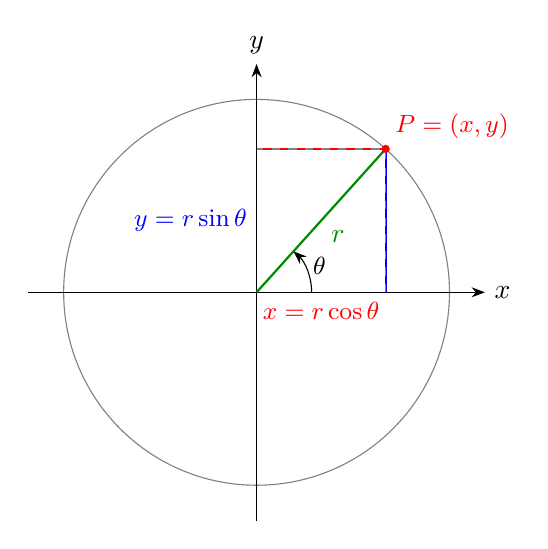
\begin{tikzpicture}[
  >=Stealth,
  guide/.style={gray,dashed,thin},
  label/.style={font=\small},
]
  \def\r{2.45}
  \def\a{48}
  \coordinate (P) at ({\r*cos(\a)},{\r*sin(\a)});
  \draw[gray] (0,0) circle (\r);
  \draw[->] (-2.9,0) -- (2.9,0) node[right] {$x$};
  \draw[->] (0,-2.9) -- (0,2.9) node[above] {$y$};
  \draw[green!55!black,thick] (0,0) -- node[below right] {$r$} (P);
  \draw[blue,thick] (P |- 0,0) -- (P);
  \draw[red,thick] (0,0 |- P) -- (P);
  \draw[guide] (P |- 0,0) -- (P) -- (0,0 |- P);
  \draw[->] (.7,0) arc[start angle=0,end angle=\a,radius=.7];
  \fill[red] (P) circle (1.5pt)
    node[above right,label] {$P=(x,y)$};
  \node[label] at (.8,.34) {$\theta$};
  \node[label,below,red] at ({\r*cos(\a)/2},0) {$x=r\cos\theta$};
  \node[label,left,blue] at (0,{\r*sin(\a)/2}) {$y=r\sin\theta$};
\end{tikzpicture}
\end{document}
